\documentclass{standalone}
\usepackage[T1]{fontenc}
\usepackage[latin2]{inputenc}
\usepackage[english]{babel}
\usepackage{tikz}
\usepackage{times}
\usetikzlibrary{calc,through,backgrounds,positioning,fit}
\usetikzlibrary{shapes,arrows,shadows,calendar}
\usetikzlibrary{lindenmayersystems}
\begin{document}
 
\centering

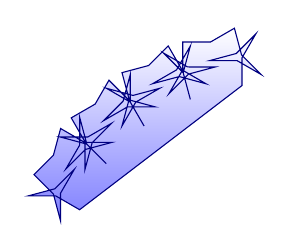
\begin{tikzpicture}
\pgfdeclarelindenmayersystem{test curve}{
\rule{A -> B++F--FB}
\rule{B -> A+A+A+A+}

}

\shadedraw [top color=white, bottom color=blue!50, draw=blue!50!black]
[l-system={test curve, step=10pt, angle=15, axiom=B, order=5}]
lindenmayer system--cycle;

\end{tikzpicture}

\end{document}